\documentclass{article}
\usepackage{arxiv}

\usepackage[utf8]{inputenc}
\usepackage[english, russian]{babel}
\usepackage[T1]{fontenc}
\usepackage{url}
\usepackage{booktabs}
\usepackage{amsfonts}
\usepackage{nicefrac}
\usepackage{microtype}
\usepackage{lipsum}
\usepackage{graphicx}
\usepackage{natbib}
\usepackage{doi}
\usepackage{amsmath}



\title{Spatiotemporal forecasting with convolutions and tensor decomposition}

\author{ David S.~Hippocampus\thanks{Use footnote for providing further
		information about author (webpage, alternative
		address)---\emph{not} for acknowledging funding agencies.} \\
	Department of Computer Science\\
	Cranberry-Lemon University\\
	Pittsburgh, PA 15213 \\
	\texttt{hippo@cs.cranberry-lemon.edu} \\
	%% examples of more authors
	\And
	Elias D.~Striatum \\
	Department of Electrical Engineering\\
	Mount-Sheikh University\\
	Santa Narimana, Levand \\
	\texttt{stariate@ee.mount-sheikh.edu} \\
	%% \AND
	%% Coauthor \\
	%% Affiliation \\
	%% Address \\
	%% \texttt{email} \\
	%% \And
	%% Coauthor \\
	%% Affiliation \\
	%% Address \\
	%% \texttt{email} \\
	%% \And
	%% Coauthor \\
	%% Affiliation \\
	%% Address \\
	%% \texttt{email} \\
}
\date{}

\renewcommand{\shorttitle}{\textit{arXiv} Template}

%%% Add PDF metadata to help others organize their library
%%% Once the PDF is generated, you can check the metadata with
%%% $ pdfinfo template.pdf
\hypersetup{
pdftitle={A template for the arxiv style},
pdfsubject={q-bio.NC, q-bio.QM},
pdfauthor={David S.~Hippocampus, Elias D.~Striatum},
pdfkeywords={First keyword, Second keyword, More},
}

\begin{document}
\maketitle

\begin{abstract}
Tensor based time series decomposition methods based on singular spectrum analysis showed great results in both denoising and interpretability. Several forecasting techniques based on them were already explored, yet none provided simultaneously accurate, stable and computationally cheap inferring. After an in-depth study of well known models we facilitated a new one comprising all three requirements for non-stationary quasi-periodic time series. The model was then tested on real-life data of electricity consumption and other well-explored datasets. 
\end{abstract}


\keywords{First keyword \and Second keyword \and More}

\section{Introduction}
Singular spectrum analysis (SSA) is a method widely used in the past decades in different areas, from economics to biology and social science [1].  One of main advantages is its ability to extract underlying frequencies from complex and multidimensional data, resulting in  variable number of components. SSA consists of two main stages: decomposition and reconstruction, both adjustable in terms of methods and hyperparameters used.

Its tensor modification (TSSA) offers [2] a more robust and accurate results by converting a series into a tensor and using  parallel factor analysis (PARAFAC) decomposition instead of the usual SVD. It optimizes usage of information initially available to a model in cost of working with more multidimensional data SSA does. The problem of reconstruction is left untouched however.

Empirical mode decomposition (EMD) can then be used  to supervise TSSA, giving us TSSA-EMD[3]. It provides a better way to identify the number of frequency components within each subspace. With such enhancement algorithms achieves [4] a distinguishable growth in accuracy of signal reconstruction with denoising, leaving other methods far behind in particular tasks.

The problem of forecasting time series has not yet being mentioned. Basic SSA shows [5] adequate results when working with series of constant-limited variation function. However it becomes highly unstable in two basic cases. With several outliers already false frequencies are extracted at decomposition stage, what does not lead to reconstruction defects but enforces unacceptable error even at earlier points of prediction. A variation growth affects SSA the same way, usually creating frequencies of much higher amplitude than are expected. That makes the early predictions seem accurate, yet giving unrealistic forecast long-wise.

To conclude, SSA is a powerful but limited method.

At the same time SSA does not utilize spatial information. Given a set of parallel time series it is meant to decompose each separately. TSSA instead can show better performance by working with them as with a whole dataset. Knowing this we experiment to determine the difference between SSA and TSSA forecasting and try to create a robust model of signal decomposition, reconstruction and prediction.
\section{Problem}
\label{sec:Problem}

\subsection{Time series}

Let \(x = \left[x_1, x_2, ..., x_n\right]\), \(x_i \in \mathbb{R}\) be a 1D time series, namely a vector. We suppose \(x\) has no trend, is quasi-periodic and it's phase trajectory is stationary.

[do we need to describe phase trajectory here?]

\subsection{Hankelization}

One of the SSA steps requires Hankelization operator \(\mathcal{H}\) to be described. With 2D matrix \(i \times j\) it works as follows:
\begin{gather}
\mathcal{H}M =
\begin{pmatrix}
	\widetilde{m}_{1} & \widetilde{m}_{2} & \dots & m_{i} \\
	\widetilde{m}_{2} & \widetilde{m}_{3} & \dots & m_{i + 1} \\
	\vdots & \vdots & \ddots & \vdots \\
	\widetilde{m}_{j} & \widetilde{m}_{j + 1} &  \dots & \widetilde{m}_{i + j - 1}
\end{pmatrix} \notag \\
\widetilde{m}_{k} = \sum_{i, j \in D_k} m_{i,j} / numD_k \\
D_k = \{(\widehat{i}, \widehat{j}) : 1 \leq \widehat{i} \leq i, 1 \leq \widehat{j} \leq j, \widehat{i} + \widehat{j} = k + 1\} \notag
\end{gather} 
For a  higher dimensional tensor \(\mathcal{H}\) performs first index wise.

\subsection{SSA}

The basic SSA consists of two stages. The first is decomposition, it maps time series to a number of components. The second is reconstruction, it combines components to frequencies of interest.

Decomposition: given a 1D vector \(x\) of size \(n\) and window size \(l\) it first creates a 2D embedding of it, a trajectory matrix \(X\) of size \(l_x \times l\):
\begin{gather}
X = [X_1, X_2, ..., X_{l}] =
 \begin{pmatrix}
	x_{1} & x_{2} & \dots & x_{l} \\
	x_{2} & x_{3} & \dots & x_{l + 1} \\
	\vdots & \vdots & \ddots & \vdots \\
	x_{l_{x}} & x_{l_x + 1} &  \dots & x_{l_x + l - 1}
\end{pmatrix} \notag \\
l_x = n - l + 1
\end{gather}

The actual value of \(l\) is chosen arbitrarily to include enough information about the signal variance.

Singular value decomposition (SVD) is then applied to \(X\) to obtain its singular values and vectors:

\begin{gather}
X = \sum \limits_{i = 1}^{d} X_i = \sum \limits_{i = 1}^{d} \sqrt{\lambda_i} u_i v_i^T
\end{gather}

Where \( \lambda_i \) is the \(i\)th eigenvalue, \(u_i\) is the corresponding left singular vector and \(v_i\) is the \(i\)th right singular vector; \(d\) is the total number of eigenvalues.

Reconstruction: given a set of components \(X_i\) it first splits them into disjoint set and sums independently:

\begin{gather}
I = \{ I_1, I_2, \dots, I_q \}, \bigsqcup \limits_{i = 1}^{q} I = \{1, 2, \dots, d\} \notag \\
X = \sum \limits_{i = 1}^{q} \hat{X}_i = \sum \limits_{i = 1}^{q} \sum \limits_{j \in I_i} X_j
\end{gather}

The choice of I is one of the most important aspects of SSA in terms of retrieving the desired frequencies.

Hankelization is then applied to \(X\) and a time series is reconstructed from it (described later).

\subsection{TSSA}

TSSA is a generalization of SSA to work with a set of parallel time series. It is based on the idea that the time series are not independent and that the information contained in one time series can be used to improve the reconstruction of another.

\subsection{Forecasting models based on SSA and TSSA}

Copypaste from [Time series SSA forecasting] tutrial link from LinkReview could be found here.

No idea on how to predict with TSSA - we are to explore this I suppose

\section{Experiment}

Preliminary experimets are currently described here. The section will be updated when the real data will be utilized.

We used sin(pi * t) + sin(e * t) to create a time series. We then applied SSA with different numbers of components taken at reconstruction step. The awaited result looks like this:

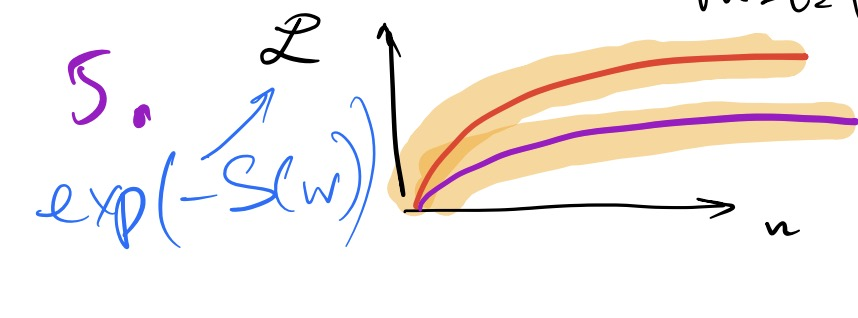
\includegraphics[scale=0.3]{./images/prelim.png}

\section{Trash}

\subsection{Citations}
Citations use \verb+natbib+. The documentation may be found at
\begin{center}
	\url{http://mirrors.ctan.org/macros/latex/contrib/natbib/natnotes.pdf}
\end{center}

Here is an example usage of the two main commands (\verb+citet+ and \verb+citep+): Some people thought a thing \citep{kour2014real, hadash2018estimate} but other people thought something else \citep{kour2014fast}. Many people have speculated that if we knew exactly why \citet{kour2014fast} thought this\dots

\subsection{Figures}
\lipsum[10]
See Figure \ref{fig:fig1}. Here is how you add footnotes. \footnote{Sample of the first footnote.}
\lipsum[11]

\begin{figure}
	\centering
	
	\caption{Sample figure caption.}
	\label{fig:fig1}
\end{figure}

\subsection{Tables}
See awesome Table~\ref{tab:table}.

The documentation for \verb+booktabs+ (`Publication quality tables in LaTeX') is available from:
\begin{center}
	\url{https://www.ctan.org/pkg/booktabs}
\end{center}


\begin{table}
	\caption{Sample table title}
	\centering
	\begin{tabular}{lll}
		\toprule
		\multicolumn{2}{c}{Part}                   \\
		\cmidrule(r){1-2}
		Name     & Description     & Size ($\mu$m) \\
		\midrule
		Dendrite & Input terminal  & $\sim$100     \\
		Axon     & Output terminal & $\sim$10      \\
		Soma     & Cell body       & up to $10^6$  \\
		\bottomrule
	\end{tabular}
	\label{tab:table}
\end{table}

\subsection{Lists}
\begin{itemize}
	\item Lorem ipsum dolor sit amet
	\item consectetur adipiscing elit.
	\item Aliquam dignissim blandit est, in dictum tortor gravida eget. In ac rutrum magna.
\end{itemize}


\bibliographystyle{unsrtnat}
\bibliography{references}

\end{document}